% Ellen
\chapter{Intrepid} \label{sec:IntroIntrepid}
Intrepid is a C++ library developed as part of Sandia's Trilinos Project.
Intrepid's main functionality is to perform algebraic operations over 
multi-dimensional arrays. Tensor
contractions are one class of operations implemented by Intrepid, widely used in
high-performance simulation software.

One particular type of tensor contraction, two-dimensional matrix
multiplication, is known to show great speedup when implemented using CPU and
especially GPU parallelism. For this reason, this clinic team considered
Intrepid tensor contractions to be good targets for parallelism, as they 
had good theoretical potential to derive
significant performance gains from parallelism.

\section{Tensor Contractions}
A tensor can be thought of as a multidimensional array. Tensor contractions are
multiplicative algebraic operations over tensors in which pairs of indices, one from each of
the two input tensors, can be ``contracted'' together, reducing the dimensionality
of the output tensor. 

As an example, three different operations can be performed on two matrices (two-dimensional tensors):
an outer product, a matrix multiplication, or an inner product. In an outer product,
the two matrices are combined to form a four-dimensional tensor. In a matrix
multiplication, two of the four resultant indices are contracted together, 
resulting in a two-dimensional tensor, a visual representation of which can be seen in Figure~\ref{fig:MatrixMultiplication}. In an inner product, all of the resultant
indices are contracted together, resulting in a scalar. In typical terminology, the last two
are considered "contractions".

\begin{figure}[h]
    \centering
    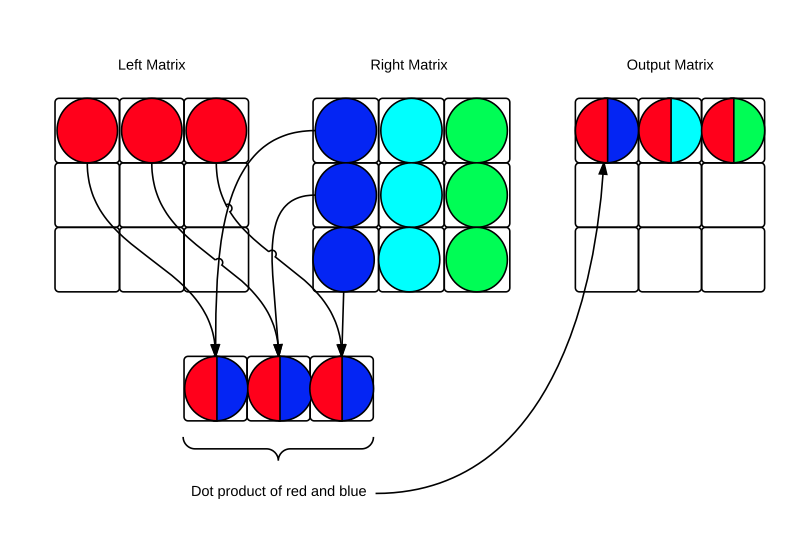
\includegraphics[scale = 0.4]{./matrix_mutiplication.png}
    \caption[Matrix multiplication]{Standard matrix multiplication. The horizontal index of the left
    matrix and the vertical index of the right matrix are contracted away.
\label{fig:MatrixMultiplication}}
\end{figure}


In this section, we have discussed the three possibilities for two-dimensional
tensor contractions. However, tensor contractions also generalize to tensors
with higher dimensionality, such as three or four dimensional tensors. In 
these higher dimensional tensors, there are more options for how many contraction 
indices might exist.

\section{Intrepid Contractions Overview}
The Intrepid library provides nine types of tensor contraction, differing by input
dimensionality, number of indices contracted away, and output dimensionality.
It is most simple to classify Intrepid's tensor contractions by number of
indices contracted away and output dimensionality.

Intrepid tensor contractions contract away one, two, or three indices. The
output of a single contraction can be a scalar (zero-dimensional), a vector
(one-dimensional), or a matrix (two-dimensional). Each combination of number of
contraction indices and output dimension is handled by one Intrepid tensor
contraction kernel.

\begin{table}[ht]
        \begin{tabular} {| l | l | l | l |l |}
            \hline
            \textbf{Kernel Name} & \textbf{Left Input} & \textbf{Right Input} &
            \textbf{Output} & \textbf{Contraction Indices}\\
            \hline
            ContractDataDataScalar   & 1D & 1D & Scalar & One \\
            ContractDataDataVector   & 2D & 2D & Scalar & Two \\
            ContractDataDataTensor   & 3D & 3D & Scalar & Three \\
            ContractDataFieldScalar  & 2D & 1D & Vector & One \\
            ContractDataFieldVector  & 3D & 2D & Vector & Two \\
            ContractDataFieldTensor  & 4D & 3D & Vector & Three \\
            ContractFieldFieldScalar & 2D & 2D & Matrix & One \\
            ContractFieldFieldVector & 3D & 3D & Matrix & Two \\
            ContractFieldFieldTensor & 4D & 4D & Matrix & Three \\
            \hline
        \end{tabular}
\caption{Summary of the nine Intrepid tensor contraction kernels
\label{tab:IntrepidContractionSummary}}
\end{table}

In order to more easily discuss specific tensor contraction kernels in Intrepid,
it helps to first understand the naming convention used for the kernel names.
Each kernel's name contains two suffixes, where the first indicates the
dimensionality of the output and the second indicates the number of contraction
indices.

\begin{table}[ht]
    \begin{center}
        \begin{tabular} {| l | l | l |}
            \hline
            \textbf{String} & \textbf{Position} & \textbf{Meaning} \\
            \hline
            DataData    & First Suffix  & Scalar Output    \\
            DataField   & First Suffix  & Vector Output    \\
            FieldField  & First Suffix  & Matrix Output    \\
            Scalar      & Second Suffix & One Contraction Index \\
            Vector      & Second Suffix & Two Contraction Indices \\
            Tensor      & Second Suffix & Three Contraction Indices \\
            \hline
        \end{tabular}
    \end{center}
\caption{Intrepid tensor contraction suffixes
\label{tab:IntrepidNamingConvention}}
\end{table}

For instance, in the \texttt{ContractDataDataScalar} kernel, the first suffix
\texttt{DataData} is used for kernels that produce scalar outputs, and the
second suffix \texttt{Scalar} is used for kernels that contract away one
dimension. Therefore, the Intrepid kernel \texttt{ContractDataDataScalar}
produces scalar outputs and contracts away one dimension, and so by necessity
the inputs for a single contraction must be vectors (one-dimensional tensors). All of the Intrepid tensor
contraction kernel suffixes are summarized in
Table~\ref{tab:IntrepidNamingConvention}. The nine tensor contractions in
Intrepid are summarized in Table~\ref{tab:IntrepidContractionSummary}.

It is also important to note that the tensor contraction kernels in Intrepid each actually perform many
contractions. For instance, \texttt{ContractDataDataScalar}, which performs
contractions of two input vectors to a single output scalar (commonly known as a dot product),
actually calculates an array of dot products. That is, the inputs are both
arrays of vectors, and the output is an array of scalars. This is represented
in the code using a dummy index, which we call the \texttt{Cell} index.

\section{ContractDataDataScalar}
\texttt{ContractDataDataScalar} is the simplest tensor contraction in Intrepid.
The kernel takes two arrays of one-dimensional tensors (vectors) and outputs an array of scalars. A
snippet showing the simple (conceptual) serial implementation of
\texttt{ContractDataDataScalar} can be seen in
Figure~\ref{lst:ContractDataDataScalarSerial}.

\begin{figure}[ht]
    \begin{lstlisting}
    for (int c = 0; c < numCells; ++c) {
      for (int qp = 0; qp < quadraturePoints; ++qp) {
        output[c] += leftInput[c][qp] * rightInput[c][qp];
      }
    }
    \end{lstlisting}
\caption{Code from serial \texttt{ContractDataDataScalar}
\label{lst:ContractDataDataScalarSerial}} 
\end{figure}

As shown in 
Figure~\ref{lst:ContractDataDataScalarSerial}, this kernel contracts away the
\texttt{Quadrature Points} dimension, leaving only the \texttt{Cell} dimension.
It can also be thought of as performing an array of dot products.

\section{ContractDataDataVector}
\texttt{ContractDataDataVector} takes two arrays of two-dimensional tensors
(matrices) and computes an array of their inner products.
\begin{figure}[ht]
    \begin{lstlisting}
    for (int c = 0; c < numCells; ++c) {
      for (int qp = 0; qp < quadraturePoints; ++qp) {
        for (int t = 0; t < iVec; ++t) {
          output[c] += leftInput[c][qp][t] * rightInput[c][qp][t];
        }
      }
    }
    \end{lstlisting}
\caption{Code from serial \texttt{ContractDataDataVector}
\label{lst:ContractDataDataVectorSerial}} 
\end{figure}

As shown in Figure~\ref{lst:ContractDataDataVectorSerial},
\texttt{ContractDataDataVector} is very similar to
\texttt{ContractDataDataScalar}, except it contracts two indices instead of
one. Again, only the \texttt{Cell} dimension is left, so we can think of this as a
sort of two-dimensional dot product.

\section{ContractDataDataTensor}\label{section:ContractDataDataTensor}
\texttt{ContractDataDataTensor} takes two arrays of three-dimensional tensors
and computes an array of their inner products.

\begin{figure}[ht]
    \begin{lstlisting}
    for (int c = 0; c < numCells; ++c) {
      for (int qp = 0; qp < quadraturePoints; ++qp) {
        for (int t1 = 0; t1 < iVec1; ++t1) {
          for (int t2 = 0; t2 < iVec2; ++t2) {
            output[c] += leftInput[c][qp][t1][t2] * 
                         rightInput[c][qp][t1][t2];
          }
        }
      }
    }
    \end{lstlisting}
\caption{Code from serial \texttt{ContractDataDataTensor}
\label{lst:ContractDataDataTensorSerial}} 
\end{figure}

As shown in Figure~\ref{lst:ContractDataDataTensorSerial},
\texttt{ContractDataDataTensor} is very similar to\\
\texttt{ContractDataDataVector} and \texttt{ContractDataDataScalar}, but has
three contraction indices instead of the one or two of the previous cases.

\section{ContractDataFieldScalar}

\texttt{ContractDataFieldScalar} takes an array of matrices and an array of
vectors and contracts away one index.

\begin{figure}[ht]
    \begin{lstlisting}
    for (int c = 0; c < numcells; ++c) {
      for (int l = 0; l < lbf; ++l) {
        for (int qp = 0; qp < quadraturepoints; ++qp) {
          output[c][l] += left[c][l][qp] * right[c][qp];
        }
      }
    }
    \end{lstlisting}
\caption{Code from serial \texttt{ContractDataFieldScalar}
\label{lst:ContractDataFieldScalarSerial}} 
\end{figure}

As shown in Figure~\ref{lst:ContractDataFieldScalarSerial},
\texttt{ContractDataFieldScalar} has two non-contraction indices, the
\texttt{Left Basis Function} index (\texttt{lbf}) and the dummy \texttt{Cell} index. The
output for this contraction is therefore an array of vectors instead of an array
of scalars.

\section{ContractDataFieldVector}
\texttt{ContractDataFieldVector} takes an array of three-dimensional tensors and
an array of vectors, and contracts away two indices to produce an array of
vectors.

\begin{figure}[ht]
    \begin{lstlisting}
    for (int c = 0; c < numcells; ++c) {
      for (int l = 0; l < lbf; ++l) {
        for (int qp = 0; qp < quadraturepoints; ++qp) {
          for (int t = 0; t < iVec; ++t) {
            output[c][l] += left[c][l][qp][t] * right[c][qp][t];
          }
        }
      }
    }
    \end{lstlisting}
\caption{Code from serial \texttt{ContractDataFieldVector}
\label{lst:ContractDataFieldVectorSerial}} 
\end{figure}

As shown in Figure~\ref{lst:ContractDataFieldVectorSerial},
\texttt{ContractDataFieldVector} is similar to \texttt{ContractDataFieldScalar},
but has two contraction indices. 

\section{ContractDataFieldTensor}
\texttt{ContractDataFieldTensor} takes an array of four-dimensional tensors and
an array of three-dimensional tensors, and contracts away two indices to produce
an array of vectors.

\begin{figure}[ht]
    \begin{lstlisting}
    for (int c = 0; c < numcells; ++c) {
      for (int l = 0; l < lbf; ++l) {
        for (int qp = 0; qp < quadraturepoints; ++qp) {
          for (int t1 = 0; t1 < iVec1; ++t1) {
            for (int t2 = 0; t2 < iVec2; ++t2) {
              output[c][l] += left[c][l][qp][t1][t2] 
                              * right[c][qp][t1][t2];
            }
          }
        }
      }
    }
    \end{lstlisting}
\caption{Code from serial \texttt{ContractDataFieldTensor}
\label{lst:ContractDataFieldTensorSerial}} 
\end{figure}

As shown in Figure~\ref{lst:ContractDataFieldTensorSerial},
\texttt{ContractDataFieldTensor} is similar to \texttt{ContractDataFieldScalar},
but has three contraction indices. 

\section{ContractFieldFieldScalar}
\texttt{ContractFieldFieldScalar} takes in two arrays of matrices and contracts
away one index to produce an array of matrices. This effectively performs classical 
matrix multiplication on each pair of input matrices.

\begin{figure}[ht]
    \begin{lstlisting}
    for (int c = 0; c < numcells; ++c) {
      for (int l = 0; l < lbf; ++l) {
        for (int r = 0; r < rbf; ++r) {
          for (int qp = 0; qp < quadraturepoints; ++qp) {
            output[c][l][r] += left[c][l][qp] * right[c][r][qp];
          }
        }
      }
    }
    \end{lstlisting}
\caption{Code from serial \texttt{ContractFieldFieldScalar}
\label{lst:ContractFieldFieldScalarSerial}} 
\end{figure}

As shown in Figure~\ref{lst:ContractFieldFieldScalarSerial},
\texttt{ContractFieldFieldScalar} has two non-contraction indices, so the output
is an array of matrices.

\section{ContractFieldFieldVector}
\texttt{ContractFieldFieldVector} takes two arrays of three-dimensional tensors
and contracts away two indices, keeping the \texttt{Cell} dummy dimension as
well as the left and right basis function indices.

\begin{figure}[ht]
    \begin{lstlisting}
    for (int c = 0; c < numcells; ++c) {
      for (int l = 0; l < lbf; ++l) {
        for (int r = 0; r < rbf; ++r) {
          for (int qp = 0; qp < quadraturepoints; ++qp) {
            for (int t = 0; t < iVec; ++t) {
              output[c][l][r] += left[c][l][qp][t] 
                                 * right[c][r][qp][t];
            }
          }
        }
      }
    }
    \end{lstlisting}
\caption{Code from serial \texttt{ContractFieldFieldVector}
\label{lst:ContractFieldFieldVectorSerial}} 
\end{figure}

As shown in Figure~\ref{lst:ContractFieldFieldVectorSerial},
\texttt{ContractFieldFieldVector} is similar to
\texttt{ContractFieldFieldScalar}, but with two contraction indices.

\section{ContractFieldFieldTensor}
\texttt{ContractFieldFieldTensor} is the most complex (in terms of number of 
input indices) of the tensor contraction
kernels in Intrepid. This kernel takes two arrays of four-dimensional tensors and
and contracts away three indices, keeping the \texttt{Cell} dummy dimension as
well as the left and right basis function indices.

\begin{figure}[ht]
    \begin{lstlisting}
    for (int c = 0; c < numcells; ++c) {
      for (int l = 0; l < lbf; ++l) {
        for (int r = 0; r < rbf; ++r) {
          for (int qp = 0; qp < quadraturepoints; ++qp) {
            for (int t1 = 0; t1 < iVec1; ++t1) {
              for (int t2 = 0; t2 < iVec2; ++t2) {
                  output[c][l][r] += left[c][l][r][qp][t1][t2] 
                                     * right[c][l][r][qp][t1][t2];
              }
            }
          }
        }
      }
    }
    \end{lstlisting}
\caption{Code from serial \texttt{ContractFieldFieldTensor}
\label{lst:ContractFieldFieldTensorSerial}} 
\end{figure}

As shown in Figure~\ref{lst:ContractFieldFieldTensorSerial},
\texttt{ContractFieldFieldTensor} is similar to
\texttt{ContractFieldFieldScalar}, but with three contraction indices.

